\section{Definiowanie rozmaitości}

\subsection{Rozmaitość topologiczna}

\begin{definition}[przestrzeń topologiczna]
  Przestrzeń topologiczna $M$ jest $n$-wymiarową rozmaitością ($n$-rozmaitością) topologiczną, jeśli:
  \begin{itemize}
    \item jest \acc{Hausdorffa}
    \item ma \acc{przeliczalną bazę} topologii
    \item jest \acc{lokalnie euklidesowa} wymiaru $n$, tzn. każdy punkt posiada otoczenie otwarte homeomorficzne z otwartym podzbiorem w $\R^n$
  \end{itemize}
\end{definition}

  Warunkiem równoważnym do lokalnej euklidesowości jest posiadanie przez każdy punkt $p\in M$ otoczenia $U$ takiego, że istnieje homeomorfizm $U\xrightarrow[]{\cong} B_r\subseteq\R^n$. [ćwiczenia]
  \bigskip

\textbf{Hausdorffowość}

Dzięki warunkowi Hausdorffowości wykluczone są np. patologie pokroju

\begin{illustration}
  \draw(0, 0)--(2, 0);
  \draw[orange] (1.2, -0.02)--(2, -0.02);
  \draw[orange] (2, -0.52)--(2.8, -0.52);

  \draw[green] (1.5, 0.02)--(2, 0.02);
  \draw[green] (2, 0.52)--(2.5, 0.52);


  \filldraw[color=black, fill=white] (2, 0) circle (1.5pt);
  \draw (2, 0.5)--(4, 0.5);
  \filldraw (2, 0.5) circle (1.5pt) node [above] {$A$};
  \draw(2, -0.5)--(4, -0.5);
  \filldraw(2, -0.5) circle (1.5pt) node [below] {$B$};
  
  \draw[green, very thick] (1.6, 0.2) arc (120:240:0.2);
  \draw[orange, very thick] (1.3, 0.2) arc (120:240:0.2);


  \draw[green, very thick] (2.4, 0.7) arc (60:-60:0.2);
  \draw[orange, very thick] (2.7, -0.3) arc (60:-60:0.2);
\end{illustration}

gdzie punktów $A$ i $B$ nie da się rozdzielić za pomocą rozłącznych zbiorów otwartych.

Ogólniej, warunek ten mówi, że lokalnie topologiczne własności z $\R^n$ przenoszą się na $M$ przez homeomorfizmy, np dla podzbioru $U\subseteq M$ i homeomorfizmu $\phi:U\to\overline{U}\subseteq\R^n$:

\begin{illustration}
%\draw[help lines,step=1] (0, 0) grid (12,4);
\draw[rounded corners=36pt](6,-1)--(4.2,-1)--(2,-2)--(0,0)--(2,2)--(4.2,1)--(7,1)--(9.2,2)--(11,0)
--(9,-2)--(6,-1);
\draw (1.5,0.2) arc (175:315:1cm and 0.5cm);
\draw (3,-0.28) arc (-30:180:0.7cm and 0.3cm);
%\draw (5.8,0) arc (0:360:0.5cm and 1cm);
\draw (7.5,0.2) arc (175:315:1cm and 0.5cm);
\draw (9,-0.28) arc (-30:180:0.7cm and 0.3cm);
%\node (a) at (-13:5.8) {$\partial M$};
%\node (a) at (26:2.5) {$\tilde{M}$};
\draw[rotate around={20:(4.5, 0)}] (4.5, 0) ellipse (0.5 and 0.8) node [below] {$U$};
\filldraw (4.3, 0.2) circle (1.5pt) node [below] {$p$};
\draw[->] (10, 2) node [right] {$\R^n$} --(10, 4);
\draw[->] (9, 3) --(11, 3);
\draw (10, 3) circle (0.7);
\node at (11, 3.8) {$\overline{U}=\phi(U)$};
\draw[smooth, ->, tension=1] plot coordinates {(5, 0.3) (6, 0.4) (8, 1.2) (9.3, 2.5)};
\node at (8.3, 1.1) {$\phi$};
\end{illustration}

Dodatkowo, dla dowolnego \emph{zwartego} $\overline K\subseteq\overline{U}$ jego odpowiednik na $M$, czyli $K=\phi^{-1}(\overline{K})\subseteq U$, jest \emph{domknięty i zwarty} [ćwiczenia]. Jeśli zaś $\overline{K}$ jest zbiorem domknięty w $\overline{U}$, ale niezwartym, to nie zawsze $K$ jest domknięty w $M$. Weźmy np. $\phi:U\to\overline{U}=\R^n$ i zbiór domknięty $\overline{K}=\R^n$ (cała przestrzeń jest jednocześnie domknięta i otwarta). Wtedy $K=\phi^{-1}(\overline{K})=U$ jest otwartym podzbiorem  $M$ mimo, że $\overline{K}$ jest otwarte.

Skończone podzbiory rozmaitości będącej przestrzenią Hausdorffa są zawsze domknięte i co ważne, granice ciągów na rozmaitościach topologicznych są jednoznacznie określone.
\medskip

\textbf{Przeliczalna baza}

Warunek przeliczalnej bazy został wprowadzony, by rozmaitości nie były "zbyt duże". Nieprzeliczalna suma parami rozłącznych kopii $\R^n$ nie może być rozmaitością. Warunek ten implikuje, że każde pokrycie zbiorami otwartymi zawiera przeliczalne podpokrycie [ćwiczenia], co jest nazywane \important{warunkiem Lindel\"ofa}.

Przeliczalność bazy implikuje również, że każda rozmaitość topologiczna jest wstępującą sumą zbiorów otwartych
$$U_1\subseteq U_2\subseteq...\subseteq U_n\subseteq...,$$
które po domknięciu są nadal zawarte w niej. Pozwala ona również na włożenie $M$ do $\R^n$ dla odpowiednio dużego $n$. Czyli na przykład $S^2$, sfera, ma naturalne włożenie w $\R^3$ pomimo lokalnej euklidesowości z $\R^2$.

Rodzina $\set{X}$ podzbiorów $M$ jest \acc[i]{lokalnie skończona}, jeżeli każdy punkt $p\in M$ ma otoczenie, które przecina się co najwyżej ze skończoną liczbą zbiorów z $\set{X}$. Jeżeli $M$ ma dwa pokrycia: $\set{U}$ i $\set{V}$ takie, że dla każdego $V\in\set{V}$ znajdziemy $U\in\set{U}$ takie, że $V\subseteq U$, to $\set{V}$ jest \acc[i]{pokryciem włożonym/rozdrobnieniem} $\set{U}$. Dzięki przeliczalności bazy $M$, każda rozmaitość jest \important{parazwarta}, czyli zawiera lokalnie skończone rozdrobnienie.

\textbf{Lokalna euklidesowość}

\begin{theorem}[twierdzenie brouwer'a]\label{twierdzebie brouwer'a} \textbf{\color{orange}Twierdzenie Brouwer'a} Dla $m\neq n$ otwarty podzbiór $\R^n$ nie może być homeomorficzny z żadnym otwartym podzbiorem $\R^m$.
\end{theorem}

\marginpar{Tutaj warto zaznaczyć, że zbiór pusty zaspokaja definicję rozmaitości topologicznej dla dowolnego $n$. Wygodnie jest go jednak móc użyć, więc w definicji niepustość $M$ nie jest przez nas wymagana.}Z twierdzenia wyżej wynika, że liczba $n$ jest przypisana do $M$ jednoznacznie i nazywa się \important{wymiarem} $M$ ($dim(M)=n$). Jeśli wymiar rozmaitości $M$ wynosi $n$, to nazywamy ją czasem \acc[i]{$n$-rozmaitością}.
\bigskip

\textbf{\large Inne własności rozmaitości topologicznych:}
\begin{itemize}
  \item Każda rozmaitość ma przeliczalną bazę złożoną ze zbiorów homeomorficznych z kulami w $\R^n$, których domknięcia są zbiorami zwartymi.
  \item Każda rozmaitość jest lokalnie spójna, tzn. ma bazę otwartych zbiorów łukowo spójnych.
  \item Rozmaitość jest spójna $\iff$ jest łukowo spójna. Składowe spójności $M$ są równe składowym łukowej spójności $M$.
  \item Każda rozmaitość jest lokalnie zwarta (tzn. każdy punkt posiada zwarte otoczenie).
\end{itemize}

\subsection{Mapy, współrzędne lokalne}

\begin{definition}[mapa]
  \important{Mapą} na rozmaitości topologicznej $M$ nazywamy parę $(U, \phi)$, gdzie $U$ jest otwartym podzbiorem $M$, zaś $\phi:U\to\overline{U}=\phi(U)\subseteq\R^n$ jest homeomorfizmem na otwarty podzbiór w $\R^n$. Zbiór $U$ nazywamy wtedy \acc[b]{zbiorem mapowym}
\end{definition}

Ponieważ każda rozmaitość topologiczna jest lokalnie euklidesowa, to $M$ jest pokrywana zbiorami mapowymi. 

Dla mapy $(U, \phi)$ takiej, że $p\in U$ i $\phi(p)=0\in\R^n$ mówimy, że jest \acc[i]{mapą wokół $p$}. Za pomocą translacji możemy każdą mapę zawsze przesunąć tak, aby $\phi(p)=0$. Czyli możemy odgórnie zakładać, że mapa $(U,\phi)$ jest mapą o początku w $p$.

Często będziemy przechodzić do coraz to mniejszych zbiorów mapowych poprzez branie odwzorowań obciętych co nie burzy gładkości ani zgodności z atlasem. Pozwoli to np. zakładać, że dla $p\notin F$ domkniętego bierzemy mapę $(U,\phi)$ taką, że $U\cap F=\emptyset$.

Mapy nazywa się też czasem \acc[i]{lokalnymi współrzędnymi} na $M$ lub \acc[i]{lokalną parametryzacją} $M$. Ponieważ o mapie można myśleć jako o przeniesieniu siatki współrzędnych $(x_1,...,x_n)$ z $\overline{U}=\phi(U)$ przez $\phi^{-1}$ na $U$, to będziemy często utożsamiać $U\subseteq M$ z $\overline{U}$. O punkcie $p\in M$ takim, że $\phi(p)=(x_1,...,x_n)$ będziemy myśleć jako o $p=(x_1,...,x_n)$.

\begin{illustration}
%\draw[help lines,step=1] (0, 0) grid (12,4);
\draw[rounded corners=36pt](6,-1)--(4.2,-1)--(2,-2)--(0,0)--(2,2)--(4.2,1)--(7,1)--(9.2,2)--(11,0)
--(9,-2)--(6,-1);
\draw (1.5,0.2) arc (175:315:1cm and 0.5cm);
\draw (3,-0.28) arc (-30:180:0.7cm and 0.3cm);
%\draw (5.8,0) arc (0:360:0.5cm and 1cm);
\draw (7.5,0.2) arc (175:315:1cm and 0.5cm);
\draw (9,-0.28) arc (-30:180:0.7cm and 0.3cm);
%\node (a) at (-13:5.8) {$\partial M$};
%\node (a) at (26:2.5) {$\tilde{M}$};
\filldraw[rotate around={20:(4.5, 0)}, pattern={Hatch[angle=20, distance=5pt]}] (4.5, 0) ellipse (0.5 and 0.8);
%\filldraw (4.3, 0.2) circle (1.5pt) node [below] {$p$};
\draw[->] (10, 2) node [right] {$\R^n$} --(10, 4);
\draw[->] (9, 3) --(11, 3);
\draw[pattern={Hatch[distance=5pt]}] (10, 3) circle (0.7);
%\node at (11, 3.8) {$\overline{U}=\phi(U)$};
\draw[smooth, ->, tension=1] plot coordinates {(5, 0.3) (6, 0.4) (8, 1.2) (9.3, 2.5)};
\node at (8.3, 1.1) {$\phi$};
\end{illustration}
\bigskip

\begin{example}
\item Każdy otwarty podzbiór $n$-rozmaitości topologicznej jest $n$-rozmaitością [ćwiczenia].
    \item \textbf{Wykresy ciągłych funkcji}: Niech $U\subseteq\R^n$ i $f:U\to\R^k$ jest funkcją ciągłą. Wykresem $f$ nazywamy zbiór 
      $$\Gamma(f)=\{(x, y)\;:\;x\in U,\;y=f(x)\}\subseteq\R^n\times\R^k$$
      Oznaczmy przez $\pi_1:\R^n\times\R^k\to\R^n$ projekcję na $\R^n$, tzn. $\pi_1(x, y)=x\in\R^n$. Wtedy funkcja $\phi:\Gamma(f)\to U$ będąca obcięciem $\pi_1$ do $\Gamma(f)$. Ponieważ $\phi$ jest obcięciem funkcji ciągłej, to samo również jest ciągłe. W dodatku, funkcja $\phi^{-1}:\R^n\to\Gamma(f)$ dana przez $\phi^{-1}(x)=(x, f(x))\in\Gamma(f)$, jest ciągłą funkcją odwrotną do $\phi$. W takim razie, $\phi$ jest homeomorfizmem między $U$ a $\Gamma(f)$ i wykres funkcji ciągłych jest lokalnie euklidesowy. Jako podzbiór $\R^n\times\R^k$ jest też przestrzenią Hausdorffa oraz ma przeliczalną bazę. W takim razie, wykres ciągłej funkcji jest rozmaitością topologiczną.
    \item Sfery $S^n$ są $n$-rozmaitościami, które wkładają się w $\R^{n+1}$ ($S^n=\{(x_1,...,x_{n+1})\in\R^{n+1}\;:\;\sum x_i^2=1\}$).

\begin{illustration}
    \shade[ball color=yellow, opacity=0.3] (2.3,0.3) arc (0:-180:2.3 and 0.6) arc (180:0:2.3 and 2.3);
    \shade[ball color=green, opacity=0.3] (2.3, -0.3) arc (0:-180:2.3 and 2) arc (180:0:2.3 and 0.6);
    \draw[color=yellow, opacity=0.5] (2.3,0.3) arc (0:-180:2.3 and 0.6) arc (180:0:2.3 and 2.3);
    \draw[color=green, opacity=0.5] (2.3, -0.3) arc (0:-180:2.3 and 2);
    \draw[color=green, opacity=0.5] (2.3, -0.3) arc (0:-180:2.3 and 0.6);
    \draw (0,0) circle (2);
    \draw (-2,0) arc (180:360:2 and 0.6);
    \draw[dashed] (2,0) arc (0:180:2 and 0.6);
    \node at (2.5, 2) {$\color{yellow}U_i^+\cap S^n$};
    \node at (2.5, -2) {$\color{green}U_i^-\cap S^n$};

    \draw (-2,-4) arc (180:360:2 and 0.6);
    \draw[dashed] (2,-4) arc (0:180:2 and 0.6);
    %\draw (-3, -5)--(3, -3);
    %\draw (-3, -4)--(3, -4);
    \draw[->] (0, -2.5)--(0, -3) node [midway, left] {$\phi_i^\pm$};
\end{illustration}
  
      Rozważmy rodzinę par $\{(U_i^{\pm},\phi^{\pm}_i)\;:\;i=1,...,n+1\}$ na $S^n$ zdefiniowanych jako:
      $$U_i^+=\{x\in S^n\;:\;x_i>0\}$$
      $$U_i^-=\{x\in S^n\;:\;x_i<0\}$$
      \marginpar{Oznaczenie $\hat{x_i}$ oznacza "wyrzucenie" danej współrzędnej.}
      $$\phi_i^{\pm}(x)=(x_1,...,x_{i-1},\hat{x_i},x_{i+1},...,x_n).$$
      Zbiory $U_i^\pm$ pokrywają całe $S^n$, gdyż każdy punkt posiada co najmniej jedną niezerową współrzędną, a funkcje $\phi_i^\pm$ są ciągłe jako obcięcia rzutów $\R^{n+1}$ na $\R^n$. Obrazem zbioru $U_i^{\pm}$ przez $\phi_i^\pm$ jest zbiór
      $$\overline{U_i^\pm}=\phi_i^\pm(U_i^\pm)=\{(x_1,...,x_n)\;:\;\sum x_i^2<1\}$$
      czyli otwarta kula w $\R^n$.

      Odwzorowania $\phi_i^\pm$ są bijekcjami o odwzorowaniach odwrotnych:
      $$(\phi_i^\pm)^{-1}(x_1,...,x_n)=(x_1,...,x_{i-1}, \pm\sqrt{1-\sum x_i^2},x_i,...,x_n)$$
      które są ciągłe. W takim razie $\phi_i^\pm$ są homeomorfizmami między otwartymi podzbiorami $S^n$ a otwartymi podzbiorami $R^n$.

      Pokazaliśmy lokalną euklidesowość $S^n$, natomiast bycie przestrzenią Hausdorffa o przeliczalnej bazie $S^n$ dziedziczy z $\R^{n+1}$.
      
    \item Produkt kartezjański dwóch (lub $k$) rozmaitości topologicznych rozmaitością topologiczną [ćwiczenia].
    \item $n$-torus jest przestrzenią produktową $\mathds{T}^n=S^1\times...\times S^1$ i $n$-rozmaitością topologiczną. $\mathds{T}^2$ nazywamy po prostu torusem.
\end{example}


\subsection{Rozmaitości gładkie (różniczkowalne)}

Dla funkcji $f:M\to \R$ chcemy rozpoznawać je różniczkowalność za pomocą map $(U, \phi)$ na $M$.

\begin{wrapfigure}{r}{5.5cm}
\centering
\scalebox{0.8}{
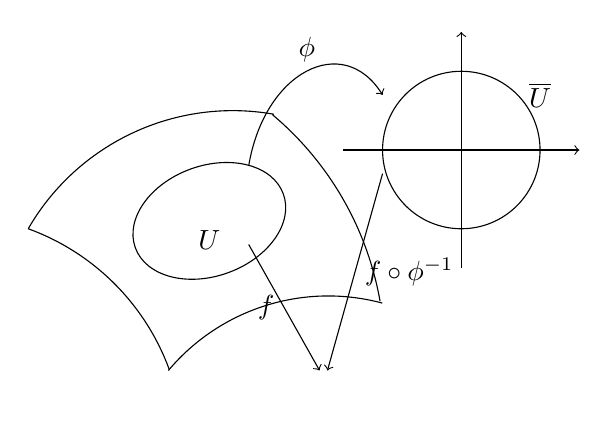
\begin{tikzpicture}
  \draw (0, 0) arc (150:80:3);
  \draw (3.1, 1.45) arc (50:10:4);
  \draw (0, 0) arc (70:20:3);
  \draw (1.78, -1.8) arc (140:75:2.65);

  \draw[rotate around={20:(2.3, 0.1)}] (2.3, 0.1) ellipse (1 and 0.7) node [below] {$U$};

  \draw[->] (4, 1)--(7, 1);
  \draw[->] (5.5, -0.5)--(5.5, 2.5);
  \draw (5.5, 1) circle (1);
  \node at (6.5, 1.7) {$\overline{U}$};
  \draw[->] (2.8, 0.8)..controls(3, 2)and(4, 2.5)..(4.5, 1.7) node [midway, above] {$\phi$};
  \draw[->] (4.5, 0.7)--(3.8, -1.8) node [midway, right] {$f\circ\phi^{-1}$};
  \draw[->] (2.8, -0.2)--(3.7, -1.8) node [midway, left] {$f$};
  \node at (3.75, -2) {$\R$};
\end{tikzpicture}
}
\end{wrapfigure}
Funkcja $f:M\to\R$ \important{wyrażona w mapie} $(U,\phi)$ to złożenie $f\circ\phi^{-1}:\overline{U}\to \R$.

\begin{definition}[funkcja $f:M\to\R$ jest gładka] Funkcja $f:M\to \R$ jest \important{gładka}, jeśli dla każdej mapy $(U, \phi)$ na $M$ $f\circ\phi^{-1}$ jest gładka.
\end{definition}

W tej definicji pojawia się pewien problem: dla jednej mapy $(U, \phi)$ $f$ może gładka, ale jeśli przejdziemy z obrazu mapy $(U, \psi)$ to może się okazać, że $f_2=f_1\circ\psi\circ\phi^{-1}$ nie jest gładka:

\begin{illustration}
  \draw (0, 0) arc (150:80:3);
  \draw (3.1, 1.45) arc (50:10:4);
  \draw (0, 0) arc (70:20:3);
  \draw (1.78, -1.8) arc (140:75:2.65);

  \draw[rotate around={20:(2.3, 0.1)}] (2.3, 0.1) ellipse (1 and 0.7) node [below] {$U$};

  \draw[->] (6, 1)--(9, 1);
  \draw[->] (7.5, -0.5)--(7.5, 2.5);

  \draw (7.5, 1) circle (1);
  \node at (8.5, 1.7) {$\overline{U}$};
  \draw[->] (2.8, 0.8)..controls(4, 2)and(5, 2.5)..(6.5, 1.7) node [midway, above] {$\phi$};
  \draw[->] (6.5, 0.5)--(2.9, -2.1) node [midway, right] {$f_1=f\circ\phi^{-1}$};
  \draw[->] (2.8, -0.2)--(2.8, -2) node [midway, left] {$f$};

  \draw[->] (-1, 1)--(-4, 1);
  \draw[->] (-2.5, -0.5)--(-2.5, 2.5);

  \draw (-2.5, 1) circle (1);
  \node at (-3.5, 1.7) {$\overline{\overline{U}}$};
  \draw[->] (-1.5, 0.5)--(2.7, -2.1) node [midway, left] {$f_2=f\circ\psi^{-1}$};
  \draw[->] (1.7, 0.5)..controls(1, 2)and(-1, 2.5)..(-1.5, 1.7) node [midway, above] {$\psi$};

  \node at (2.8, -2.3) {$\R$};

  \draw[<-] (-2, 2.3)..controls(0, 3.5)and(5, 3.5)..(7, 2.3) node [midway, above] {$\psi\circ\phi^{-1}$};
\end{illustration}

Dlatego chcemy móc założyć, że $\phi\circ\psi^{-1}$ jest przekształceniem gładkim.

\begin{definition}[zgodność map]
  Mapy $(U, \phi), (V, \psi)$ nazywamy (gładko) \important{zgodnymi}, gdy $\phi\circ\psi^{-1}$ i $\psi\circ\phi^{-1}$ są odwzorowaniami gładkimi.
\end{definition}

Odwzorowania $\phi\psi^{-1}$ nazywamy \acc[i]{odwzorowaniami przejścia} z jednej mapy do drugiej. Jeśli $\phi\psi^{-1}$ i $\psi\phi^{-1}$ są gładkie, to są one wzajemnie do siebie odwrotnymi bijekcjami. Takie odwzorowania nazywamy \acc[b]{dyfeomorfizmami} pomiędzy otwartymi podzbiorami $\R^n$. Zauważmy, że w każdym punkcie Jakobian, czyli wyznacznik macierzy pochodnych cząstkowych, jest dla dyfeomorfizmów niezerowy [ćwiczenia].

W ogólnym przypadku, gdy $U\cap V\neq \emptyset$, rysunek wygląda:
\begin{illustration}
  \draw (0, 0) arc (150:80:3);
  \draw (3.1, 1.45) arc (50:10:4);
  \draw (0, 0) arc (70:20:3);
  \draw (1.78, -1.8) arc (140:75:2.65);


  \filldraw[color=white, pattern=grid] (2.3, 0.65)--(2.4, 0.65)--(2.56, 0.55)--(2.57, 0.4)--(2.53, 0.3)--(2.3, 0.1)--(2.06, 0.3)--(2.03, 0.4)--(2.04, 0.55)--(2.2, 0.65)--cycle;
  \node at (2.3, 0.8) {$\scriptstyle U\cap V$};

  \draw[rotate around={20:(2, 0.3)}] (2, 0.3) ellipse (0.6 and 0.3);
  \node at (1.2, 0) {$V$};

  \draw[rotate around={-20:(2.6, 0.3)}] (2.6, 0.3) ellipse (0.6 and 0.3);
  \node at (3.4, 0) {$U$};

  \draw[color=white, pattern=grid] (7, 1)--(6.5, 1)--(6.6, 1.45)--(6.8, 1.75)--(7, 1.86)--cycle;
  \draw (7, 1) node [right, below] {$\scriptstyle\phi(U\cap V)$}--(7, 1.86);
  
  \draw[->] (6, 1)--(9, 1);
  \draw[->] (7.5, -0.5)--(7.5, 2.5);

  \draw (7.5, 1) circle (1);
  \node at (8.5, 1.7) {$\overline{U}$};
  \draw[->] (2.8, 0.5)..controls(4, 2)and(5, 2.5)..(6.5, 1.7) node [midway, above] {$\phi$};
  \draw[->] (6.6, 0.9)--(2.9, -2.1) node [midway, right] {$f_1=f\circ\phi^{-1}$};
  \draw[->] (2.8, -0.2)--(2.8, -2) node [midway, left] {$f$};

  \draw[color=white, pattern=grid] (-2, 1)--(-1.5, 1)--(-1.6, 1.45)--(-1.8, 1.75)--(-2, 1.86)--cycle;
  \draw (-2, 1)node [left, below] {$\scriptstyle\psi(U\cap V)$}--(-2, 1.86);

  \draw[->] (-1, 1)--(-4, 1);
  \draw[->] (-2.5, -0.5)--(-2.5, 2.5);

  \draw (-2.5, 1) circle (1);

  \node at (-3.5, 1.7) {$\overline{V}$};
  \draw[->] (-1.6, 0.95)--(2.7, -2.1) node [midway, left] {$f_2=f\circ\psi^{-1}$};
  \draw[->] (1.7, 0.5)..controls(1, 2)and(-1, 2.5)..(-1.5, 1.7) node [midway, above] {$\psi$};

  \node at (2.8, -2.3) {$\R$};

  \draw[<-] (-2, 2.3)..controls(0, 3.5)and(5, 3.5)..(7, 2.3) node [midway, above] {$\psi\circ\phi^{-1}:\phi(U\cap V)\to\psi(U\cap V)$};
\end{illustration}

  Mapy $(U, \phi)$ i $(V, \psi)$ nazywamy zgodnymi, jeśli:
  \begin{itemize}
    \item $U\cap V=\emptyset$
    \item odwzorowania przejścia 
      $$\phi\psi^{-1}:\psi(U\cap V)\to\phi(U\cap V)$$ 
      oraz 
      $$\psi\phi^{-1}:\phi(U\cap V)\to\psi(U\cap V)$$
      są gładkie ($\iff$ są dyfeomorfizmami podzbiorów $\phi(U\cap V)$ i $\psi(U\cap V)$).
  \end{itemize}

\begin{definition}[atlas gładki]
  \important{Gładkim atlasem} $\set{A}$ na rozmaitości $M$ nazywamy zbiór map $\{(U_\alpha, \phi_\alpha)\}$ takich, że:
  \begin{itemize}
    \item $\{U_\alpha\}$ pokrywają całe $M$
    \item każde dwie mapy z tego zbioru są zgodne.
  \end{itemize}
\end{definition}

\begin{example}
\item Rodzina map $\{(U_i^\pm, \phi_i^\pm)\}$ na sferze $S^n$ jest atlasem gładkim na $S^n$. Dla przykładu zbadamy zgodność map $(U_i^+,\phi_i^+)$ i $(U_j^+,\phi_j^+)$ dla $i<j$.

  Popatrzmy jak wyglądają interesujące nas zbiory:
  $$U_i^+\cap U_j^+=\{x\in S^n\;:\;x_i>0, x_j>0\}$$
  $$\phi_i^+(U_i^+\cap U_j^+)=\{x\in\R^n\;:\;|x|<1, x_{j-1}>0\}$$
  bo usuwamy $i$-tą współrzędną i numery poprzednich współrzędnych spadają o $1$ w dół,
  $$\phi_j^+(U_i^+\cap U_j^+)=\{x\in\R^n\;:\;|x|<1, x_i>0\}$$
  bo w tym przypadku usunęliśmy współrzędną na prawo od $i$, więc jej położenie nie zmienia się.
  \begin{figure}[h!]
    \begin{illustration}
      \filldraw[color=black, fill=blue!40] (-3, 0) arc (180:0:3cm);
      \filldraw[color=blue!40, fill=blue!40](-3, 0.02) arc (180:360:3cm and 1cm);
      \filldraw[color=black, fill=blue!40] (0, 3) arc (90:-90:3cm);
      \filldraw[color=blue!40, fill=blue!40] (0.02, 3) arc (90:270: 1cm and 3cm);
      \filldraw[color=black, fill=green!40] (3, 0) arc (0:90:3cm);
      \filldraw[color=black, fill=green!40] (0, 3) arc (90:200:1cm and 3cm);
      \filldraw[color=black, fill=green!40] (3, 0) arc (0:-110:3cm and 1cm);
      \filldraw[color=green!40, fill=green!40] (0, 3)--(3, 0)--(-1, -1)--cycle;

      \node at (3, 2) {$U_i^+\cap U_j^+$};

      \draw (0,0) circle (3cm);
      \draw (-3,0) arc (180:360:3cm and 1cm);
      \draw[dashed] (-3,0) arc (180:0:3cm and 1cm);
      \draw (0,-3) arc (270:90:1cm and 3cm);
      \draw[dashed] (0,3) arc (90:-90:1cm and 3cm);

      \filldraw[blue!40] (-4, -5) arc (180:90:1.5);
      \filldraw[blue!40] (-4, -5)--(-2.5, -5)--(-2.5, -3.5)--cycle;
      \filldraw[green!40] (-1, -5) arc (0:90:1.5);
      \filldraw[green!40] (-1, -5)--(-2.5, -5)--(-2.5, -3.5)--cycle;
      \draw[<-, thick] (-2.5, -3)--(-2.5, -7);
      \draw[->, thick] (-4.5, -5)--(-0.5, -5);
      \draw (-2.5, -5) circle (1.5);

      \filldraw[blue!40] (4, -5) arc (0:-90:1.5);
      \filldraw[blue!40] (4, -5)--(2.5, -5)--(2.5, -6.5)--cycle;
      \filldraw[green!40] (4, -5) arc (0:90:1.5);
      \filldraw[green!40] (4, -5)--(2.5, -5)--(2.5, -3.5)--cycle;
      \draw[<-, thick] (2.5, -3)--(2.5, -7);
      \draw[->, thick] (4.5, -5)--(0.5, -5);
      \draw (2.5, -5) circle (1.5);

      \node (j) at (3.3, -0.8) {$U_j^+$};
      \node (i) at (-1.5, 3.3) {$U_i^+$};

      \draw[->] (i)..controls(-4, 2.5)and(-5, -2)..(-4, -4) node [midway, left] {$\phi_i^+$};
      \draw[->] (j)..controls(4, -1)and(5, -2.5)..(4, -4) node [midway, right] {$\phi_j^+$};

    \draw[->] (3, -4.5)..controls(1.5, -3.5)and(-0.5, -3.5)..(-2, -4.5) node [midway, below] {$\phi_i^+(\phi_j^+)^{-1}$};
    \end{illustration}
  \end{figure}

  \begin{center}\begin{tikzcd}
    (x_1,...,x_n)\arrow[r, "(\phi_j^+)^{-1}"]\arrow[d, sloped, phantom, "\in"] & (x_1,....,x_{j-1}, \sqrt{1-|x|^2}, x_j,...,x_n)\arrow[d, "\phi_i^+"]\\
    \{x\in\R^n\;:\;|x|<1, x_i>0\}  & (x_1,...,x_{i-1}, \hat{x_i}, x_{i+1},...,x_{j-1},\sqrt{1-|x|^2}, x_j,...,x_n)\arrow[d, sloped, phantom, "\in"]\\
                                              & \{x\in\R^n\;:\;|x|<1, x_{j-1}>0\}
  \end{tikzcd}\end{center}
  Czyli odwzorowanie przejścia jest zadane wzorem:
  $$\phi_i^+(\phi_j^+)^{-1}(x_1,...,x_n)=(x_1,...,x_{i-1},x_{i+1},...,x_{j-1},\sqrt{1-|x|^2},x_j,...,x_n)$$
  i widać, że jest ono gładkie. Pozostałe rachunki przechodzą analogicznie.

    \item Jeśli $V$ jest przestrzenią liniową wymiaru $n<\infty$ nad $\R$, to dowolna norma określona na $V$ zadaje metrykę, która pozwala określić na $V$ topologię (identyczną dla równoważnych norm). Z taką topologią $V$ jest $n$-rozmaitością z naturalnie zdefiniowaną strukturą.

      Niech $(e_1,...,e_n)$ będzie bazą $V$. Rozważmy izomorfizm $E:\R^n\to V$ zadany przez
      $$E(x)=\sum_{i\leq n}x^ie_i.$$
      Funkcja ta w kontekście topologicznym jest homeomorfizmem, więc $(V, E^{-1})$ jest mapą na $V$. 

      Jeśli $(\overline{e}_1,...,\overline{e}_n)$ jest inną bazą na $V$, to mamy homeomorfizm 
      $$\overline{E}(x)=\sum x^j\overline{e}_j$$ 
      Istnieje wtedy pewna odwracalna macierz $(A_i^j)$ taka, że 
      $$e_i=\sum A^j_i\overline{j}$$ 
      dla każdego $i$. 

      Stąd modwzorowanie przejścia między tymi dwoma mapami jest zadana przez $\overline{E}^{-1}\circ E(x)=\overline{x}$, gdzie $\overline{x}=(\overline{x}^1,...,\overline{x}^n)$ jest zadane przez
      $$\sum_{j\leq n}\overline{x}^j\overline{e}_j=\sum_{i\leq n}x^ie_i=\sum_{i,j\leq n} x^iA_i^j\overline{e}_j\implies \overline{x}^j=\sum_{i\leq n} A_i^jx^i$$

      W takim razie jakakolwiek mapa wysyłająca $x$ na $\overline{x}$ jest odwracalna i liniowa $\implies$ jest dyfeomorfizmem. Stąd dowolne dwie mapy $(V, E)$ są gładko zgodne i ich rodzina definiuje na $V$ standardową gładką strukturę.
\end{example}

\begin{definition}[rozmaitość gładka]
  \important{Rozmaitością gładką} nazywamy parę $(M, \set{A})$, gdzie $M$ jest rozmaitością topologiczną, zaś $\set{A}$ jest pewnym atlasem gładkim na $M$.
\end{definition}

Zdarza się, że różne atlasy na tej samej rozmaitości topologicznej $M$ mogą zadawać tę samą rozmaitość gładką. Na przykład dla $M=\R^n$ istnieje atlas zawierający jedną mapę $\{(\R^n, id_{\R^n})\}$ oraz atlas $\{(B_x(r), id_{B_x(r)})\;:\;x\in\R^n, r>0\}$, który jest tak naprawdę "rozdrobnieniem" pierwszego atlasu. 

\begin{definition}[zgodność atlasów, mapy z atlasem]
  Niech $\set{A}$ będzie gładkim atlasem na $M$.

  \begin{enumerate}
    \item Mapa $(U, \phi)$ jest zgodna z $\set{A}$, jeśli jest zgodna z każdą mapą $(V, \psi)\in \set{A}$.
    \item Dwa atlasy $\set{A}_1, \set{A}_2$ na $M$ są zgodne, jeśli każda mapa z $\set{A}_1$ jest zgodna z $\set{A}_2$.
  \end{enumerate}
\end{definition}

Warto zaznaczyć, że zgodność atlasów jest relacją zwrotnią i przechodnią [ćwiczenia]. Zgodne atlasy zadają tę samą strukturę rozmaitości gładkiej na topologicznej rozmaitości $M$. Wszystkie zgodne atlasy należą do jednego większego atlasu, co było przyczyną powstania definicji atlasu maksymalnego.

\begin{definition}[atlas maksymalny]
  $\set{A}$ jest \important{atlasem maksymalnym} na rozmaitości $M$, jeśli każda mapa zgodna z $\set{A}$ należy do $\set{A}$.
\end{definition}

Każdy atlas $\set{A}$ na $M$ zawiera się w dokładnie jednym atlasie maksymalnym, złożonym ze wszystkich map zgodnych z $\set{A}$ [ćwiczenia]. Dodatkowo, zgodne atlasy zawierają się w tym samym atlasie maksymalnym. Wtedy można definiować rozmaitość gładką jako parę $(M, \set{A})$, gdzie $M$ jest rozmaitością topologiczną, a $\set{A}$ jest pewnym gładkim atlasem maksymalnym.
\bigskip

\textbf{Dopowiedzenie o funkcjach gładkich}

Funkcja $f:M\to\R$ jest gładka względem atlasu $\set{A}$ na $M$, jeśli dla każdej mapy $(U, \phi)\in\set{A}$ $f\circ\phi^{-1}$ jest gładka.

\begin{fact}[gładkość względem atlasu]$ $\newline
  \begin{itemize}
    \item Jeśli $f:M\to\R$ jest gładka względem $\set{A}$, zaś $(U, \phi)$ jest mapą zgodną z $\set{A}$, to $f\circ\phi^{-1}$ jest gładka.
    \item Jeśli $\set{A}_1$ i $\set{A}_2$ są zgodnymi atlasami, to $f:M\to\R$ jest gładka względem $\set{A_1}$ $\iff$ $f$ jest gładka względem $\set{A}_2$ $\iff$ $f$ jest gładka względem atlasu maksymalnego $\set{A}_{max}$ zawierającego $\set{A}_1$ i $\set{A_2}$.
  \end{itemize}
\end{fact}
\begin{proof}
  Ćwiczenia
\end{proof}

\subsection{Warianty pojęcia rozmaitości różniczkowalnej}

Mówimy, że mapy $(U,\phi),(V, \psi)$ są \acc[i]{$C^k$-zgodne} jeśli $\phi\circ\psi^{-1}$ i $\psi\circ\phi^{-1}$ są funkcjami klasy $C^k$ (posiadają pochodne cząstkowe rzędów $\leq k$). $C^k$-atlas to z kolei rodzina $C^k$-zgodnych map, która określa strukturę $C^k$-rozmaitości na $M$. Struktura $C^k$-rozmaitości jest słabsza niż rozmaitości gładkiej i nie da się na niej zdefiniować map klasy $C^m$ dla $m>k$.

$C^0$ rozmaitość to określenie na rozmaitość topologiczną, a $C^\infty$-rozmaitość jest tym samym co rozmaitość gładka.
\medskip

\textbf{Dychotomia $C^0$ i $C^k$ dla $k>0$} aka dykresja

Z każdego maksymalnego atlasu $C^1$-rozmaitości można wybrać atlas złożony z map $C^\infty$-zgodnych. Zatem, każda $C^1$-rozmaitość posiada $C^1$-zgodną strukturę $C^\infty$-rozmaitości [Whitney, 1940]. Istnieją jednak $C^0$-rozmaitości, które nie dopuszczają żadnej zgodnej struktury gładkiej [Quinn '82, Friedmann '82].
\medskip

\begin{itemize}[leftmargin=*]
  \item Na rozmaitości analitycznej mapy są analitycznie zgodne $[C^\omega]$. Mapy są analitycznie zgodne, gdy wyrażają się za pomocą szeregów potęgowych.
  \item Rozmaitość zespolona ma mapy będące funkcjami w $\C^n$ zamiast $\R^n$.
  \item W rozmaitości konforemnej mapy zachowują kąty między punktami.
  \item Istnieją też rozmaitości kawałkami liniowe (PL)...
\end{itemize}

\subsection{Różniczkowalność odwzorowań rozmaitości}

\begin{definition}[odwzorowanie $C^k$-różniczkowalne]
Dla $M, N$ gładkich rozmaitości i $f:M\to N$ ciągłej mówimy, że $f$ jest \important{$C^k$-różniczkowalna} w punkcie $p$, jeśli dla dowolnych map $(U,\phi)\ni p$ oraz $(V,\psi)\ni f(p)$ złożenie
$$\psi\circ f\circ\phi^{-1}:\phi[U\cap f^{-1}(V)]\to \psi(V)$$
jest $C^k$-różniczkowalne w punkcie $\phi(p)$.
\end{definition}

\begin{illustration}
  \node at (0,0) {ZRÓB RYSUNEK};
\end{illustration}

\subsection{Definiowanie rozmaitości gładkiej $X$ za pomocą samego atlasu}

\begin{lemma}
  Niech $X$ będzie zbiorem (bez zadanej topologii) i $\{U_\alpha\}$ będzie kolekcją podzbiorów w $X$ taką, że dla każdego $\alpha$ istnieje $\phi_\alpha:U_\alpha\to\R^n$ różniczkowalne takie, że
  
  \begin{enumerate}
    \item dla każdego $\alpha$ $\phi_\alpha(u_\alpha)=\overline{U_\alpha}\subseteq\R^n$ jest otwarty
    \item dla dowolnych $\alpha, \beta$ $\phi_\alpha(U_\alpha\cap U_\beta)$ oraz $\phi_\beta(U_\alpha\cap U_\beta)$ są otwarte w $\R^n$.
    \item jeśli $U_\alpha\cap U_\beta\neq\emptyset$, to $\phi_\beta\circ\phi_\alpha^{-1}:\phi_\alpha(U_\alpha\cap U_\beta)\to\phi_\beta(U_\alpha\cap U_\beta)$ jest gładkie (a nawet dyfeomorficzne, bo odwzorowanie odwrotne $\phi_\alpha\circ\phi_\beta^{-a}$ też jest gładkie)
    \item przeliczalnie wiele spośród $U_\alpha$ pokrywa $X$
    \item dla każdego $p, q\in X$, jeśli $p\neq q$, to istnieją $\alpha, \beta$ oraz otwarte $V_p\subseteq\overline{U_\alpha}$ i $V_q\subseteq\overline{U_\beta}$ takie, że $p\in \phi_\alpha^{-1}(V_p), q\in\phi_\beta^{-1}(V_q)$ oraz $\phi_\alpha^{-1}(V_p)\cap\phi_\beta^{-1}(V_q)=\emptyset$ (oddzielanie punktów otwartymi zbiorami mapowymi).
  \end{enumerate}

  Wówczas na $X$ istnieje jedyna struktura rozmaitości topologicznej, dla której zbiory $U_\alpha$ są otwarte. Ponadto rodzina $\{(U_\alpha, \phi_\alpha)\}$ tworzy wtedy gładki atlas na $X$.
\end{lemma}

\begin{proof}
  A dokładniej szkic dowodu. \marginpar{Dokładny dowód w Lee, lemat 1.35.}

  Określimy topologię na $X$ przy pomocy przeciwobrazów przez $\phi_\alpha$ otwartych podzbiorów $\overline{U_\alpha}=\phi_\alpha(U_\alpha)\subseteq\R^n$. Sprawdzenie, że jest to bazą topologii jest ćwiczeniem. Dzięki temu zbadanie lokalnej euklidesowości jest trywialne.

  Dzięki warunkowi 4 nietrudno jest wybrać wtedy bazę przeliczalną [ćwiczenie], a warunek Hausdorffowości wynika z 5.
\end{proof}

\begin{example}
\item $\set{L}$ jest zbiorem prostych na płaszczyźnie. Na takim zbiorze nie ma dogodnej topologii, którą możnaby od razu wykorzystać. Zdefiniujmy zbiory:
  $$U_v=\{\text{proste niepoziome}\}$$
  $$U_h=\{\text{proste niepionowe}\}$$
  oraz funkcje $\phi_h, \phi_v$:
  $$U_h\ni L=\{y=ax+b\}\overset{\phi_h}{\mapsto} (a, b)\in\R^2$$
  $$U_v\ni L=\{x=cy+d\}\overset{\phi_v}{\mapsto} (c, d)\in\R^2$$
  Obie te funkcje są różnowartościowe i ich obrazy to $\R^2$, czyli warunek 1 jest spełniony. Ponieważ jest ich tylko 2 sztuki i pokrywają całęgo $X$, to również 4. został spełniony. Sprawdźmy teraz 2:
  $$U_h\cap U_v=\{\text{proste niepionowe i niepoziome}\}=\{y=ax+b\;:\;a\neq 0\}=\{x=cy+d\;:\;c\neq0\}$$
  $$\phi_h(U_h\cap U_v)=\{(a, b)\in\R^2\;:\;a\neq 0\}$$
  $$\phi_v(U_h\cap U_v)=\{(c, d)\;:\;c\neq0\}$$
  są otwarte, więc 2 jest spełniona. Teraz kolej na 3.
  
  Weźmy prostą $L=\{x=cy+d\}=\{y=\frac{1}{c}x-\frac{d}{c}\}\in U_h\cap U_v$. 
  \begin{center}\begin{tikzcd}
    \left(\frac{1}{c},-\frac{d}{c}\right) & \arrow[l, "\phi_h" above]L\arrow[r, "\phi_v"] & (c, d)
  \end{tikzcd}\end{center}
  Zatem $\phi_h\phi_v^{-1}(c, d)=\left(\frac1c,-\frac{d}{c}\right)$ jest gładkie (podobnie $\phi_v\phi_h^{-1}$).

  Warunek 5. jest łatwy do sprawdzenia [ćwiczenie].

  Z tą naturalną (mimo wszystko) topologią $\set{L}$ jest w istocie homeomorficzne z wnętrzem wstęgi M\"obiusa. Stąd do opisania $\set{L}$ nie wystarcza jedna mapa.
\end{example}
\bigskip

\textbf{O notacjach:}

\begin{itemize}
  \item W dalszej części rozważań będziemy utożsamiać mapowe otoczenie $U\subseteq M$ z obrazem przez mapę, czyli $\overline{U}=\phi(U)\subseteq\R^n$. Można o tym myśleć, że przenosimy siatkę współrzędnych $(x_1,...,x_n)$ z $\overline{U}$ przez $\phi^{-1}$ na $U\subseteq M$.
  \item Za pomocą translacji współrzędnych zawsze możemy przyjąć, że $p=(0,...,0)$ w mapie, czyli możemy założyć, że $(U,\phi)$ jest mapą o początku w $p$.
  \item Często będziemy przechodzić do mniejszych zbiorów mapowych, za mapę biorąc odwzorowanie obcięte (jest to mapa zgodna z atlasem). Będziemy wtedy mówić, że przyjmujemy, iż mapa wokół $p$ ma zbiór mapowy tak mały, jak nam akurat potrzeba, np. że jest rozłączny z pewnym zbiorem domkniętym $F\subseteq M$ niezawierającym $p$.
\end{itemize}

\subsection{Rozmaitość gładka z brzegiem}

\begin{bbox}
Rzeczywistą półprzestrzeń oznaczamy
$$H^n=\{(x_1,...,x_n)\in\R^n\;:\;x_n\geq 0\},$$
jej brzegiem nazywamy
$$\partial H^n=\{(x_1,...,x_n)\in\R^n\;:\;x_n=0\}$$
a wnętrzem:
$$int(H^n)=\{(x_1,..., x_n)\in\R^n\;:\;x_n>0\}.$$

Dla $U\subseteq H^n$ oznaczymy $\partial U=U\cap \partial H$ oraz $int(U)=U\cap int(H^n)$, czyli definicja brzegu i wnętrza jest nieco inna niż na topologii. Użyjemy $H^n$ oraz definicji jej brzegu i wnętrza, by zdefiniować rozmaitość gładką z brzegiem.
\end{bbox}

Dla $U\subseteq H^n$ otwartego i $f:U\to\R^m$ mówimy, że $f$ jest \important{gładka}, gdy jest obcięciem do $U$ gładkiej funkcji $\hat{f}:\hat{U}\to\R^m$, $\hat{U}\subseteq\R^n$ otwartego, $U\subseteq\hat{U}$. \emph{Pochodne cząstkowe funkcji $f$ są dobrze określone na $int(U)$, a ponieważ są ciągłe, to są również dobrze określone na $\partial U$} (tzn. nie zależą od wyboru rozszerzenia $\hat{f}$). Z analizy matematycznej wiemy, że rozszerzenia $\hat{f}$ istnieje $\iff$ wszystkie pochodne cząstkowe $f$ w $int(U)$ w sposób ciągły rozszerzają się do $\partial U$.

\begin{definition}[rozmaitość z brzegiem]
  $M$ jest \important{gładką rozmaitością z brzegiem}, jeśli posiada atlas $\{(U_\alpha,\phi_\alpha)\}$, $U_\alpha\subseteq M$ i $\phi_\alpha:U_\alpha\to H^n$ i $\overline{U_\alpha}=\phi_\alpha(U_\alpha)$ jest otwarty w $H^n$, gdzie odwzorowania przejścia są gładkie (tzn. $\phi_\alpha\phi_\beta^{-1}$ są dyfeomorfizmami pomiędzy otwartymi podzbiorami w $H^n$).
\end{definition}

\begin{illustration}
  \draw[rounded corners=35pt](7,-1)--(4.2,-1)--(2,-2)--(0,0) -- (2,2)--(4.2,1)--(7,1);
  \draw (1.5,0.2) arc (175:315:1cm and 0.5cm);
  \draw (3,-0.28) arc (-30:180:0.7cm and 0.3cm);
  \filldraw[color=blue, fill=blue!40] (6.4, 0) circle (0.6);
  \filldraw[color=black, fill=blue!40!black!60] (7.5,0) arc (0:360:0.5cm and 1cm);
  %\node (a) at (20:2.5) {$M$};
  %\node (a) at (-12:7.5) {$\partial M=N$};
  \filldraw[color=blue, fill=blue!40] (4.5, 0.35) circle (0.6);

  \filldraw[color=blue, fill=blue!40] (8.4, -0.2) circle (0.5);
  \filldraw [color=blue, fill=blue!40] (8.8, -1.5) arc (180:0:0.5);

  \draw[<-] (9, 0.5)--(9, -1.7);
  \draw[->] (7.5, -1.5)--(10.5, -1.5);

  \draw[->, white, very thick] (5, 0.4)..controls(5.5, 1.5)and(7.5, 1.3)..(8, 0);
  \draw[->, white, very thick] (6.2, -0.5)..controls(6.5, -1.5)and(8, -2)..(8.8, -1.3);

  \draw[->] (5, 0.4)..controls(5.5, 1.5)and(7.5, 1.3)..(8, 0);
  \draw[->] (6.2, -0.5)..controls(6.5, -1.5)and(8, -2)..(8.8, -1.3);

  \node at (9.4, 0.3) {$H^n$};
\end{illustration}

\begin{fact}[raz w brzegu, zawsze w brzegu]
  Jeśli w pewnej mapie $(U_\alpha,\phi_\alpha)$, $\phi_\alpha(p)\in\partial H^n$, to w każdej innej mapie $(U_\beta, \phi_\beta)$ zawierającej $p$ $\phi_\alpha(p)\in\partial H^n$.
\end{fact}

\begin{proof}
  Wynika to z twierdzenia o odwzorowaniu otwartym, wraz z nieosobliwością Jakobianu odwzorowań przejścia. 

  Dla rozmaitości topologicznych z brzegiem analogiczny fakt wymaga w dowodzie twardego twierdzenia Brouwera o niezmienniczności obrazu - analogicznego twierdzenia o odwzorowaniu otwartym dla ciągłych injekcji.
\end{proof}

\begin{definition}[brzeg, wnętrze]
  \important{Brzegiem} $n$-rozmaitości $M$ z brzegiem nazywamy zbiór
  $$\partial M=\{p\in M\;:\;\text{w pewnej (każdej) mapie }p\in(U_\alpha,\phi_\alpha)\text{ zachodzi }\phi(p)\in\partial H^n$$
    wnętrze $M$ nazywa się
    $$int(M)=\{p\in M\;:\;(\exists\;(U_\alpha,\phi_\alpha)\;\phi_\alpha(p)\in int(H^n)\}$$
\end{definition}

  \begin{fact}
    Wnętrze $int(M)$ $n$-rozmaitości gładkiej $M$ jest $n$-rozmaitością bez brzegu.
  \end{fact}

  \begin{proof}
    Jako atlas bierzemy $\{(U_\alpha',\phi_\alpha')\}$, gdzie 
    $$U_\alpha'=\phi_\alpha^{-1}(int(\overline{U_\alpha}))=U_\alpha\cap int(M),\quad\phi_\alpha'=\phi_\alpha\restriction U_\alpha'$$
    Odwzorowania przejścia $\phi_\alpha'(\phi_\beta')^{-1}$ są obcięciami $\phi_\alpha\phi_\beta^{-1}$, więc są gładkie.
  \end{proof}

\begin{example}
\item Dysk $D^n=\{x\in\R^n\;:\;|x|\leq 1\}$ jest $n$-rozmaitością z brzegiem $\partial D^n=S^{n-1}=\{x\in\R^n\;:\;|x|=1\}$.

  \begin{proof}
    Skonstruujemy mapy, pomijając sprawdzanie gładkości odwzorowań przejścia.

    Mapa $(U_0, \phi_0)$:
    $$U_0=\{x\;:\;|x|<1\},\;\phi_0:U_0\to H^n,\;\phi_0(x_1,...,x_n)=(x_1,...,x_{n-1}, x_n+2)$$

    Mapy $(U_i^\pm,\phi_i^\pm)$

    \begin{illustration}
      \filldraw[green!40] (0, 1.5) arc (90:-90:1.5);
      \draw (0, 0) circle (1.5);
      \draw (1.5, -2)--(1.5, 2);
      \filldraw (0.8, -0.5) circle (1.5pt) node [below] {p};
      \draw (0, 0)--(1.5, -0.95);
      \filldraw (1.5, -0.95) circle (1.5pt) node [right] {$\pi(p)$};
      \filldraw (0,0)circle(1.5pt);
      \draw(0, 1.5)--(0, -1.5);
      \node at (3, -1.5) {$\R^{n-1}=\{x_i=1\}$};
      \node at (-1, -1.5) {$D^n$};
      \node (a) at (-0.5, 2) {$U_i^\pm$};
      \draw (-0.3, 1.8)--(0.4, 1);
    \end{illustration}
    $$U_i^+=\{x\in D^n\;:\;x_i>0\}$$
    $$U_i^-=\{x\in D^n\;:\;x_i < 0\}$$
    $$\phi_i^\pm(x_1,...,x_n)=\left(\frac{x_1}{x_i},...,\frac{x_{i-1}}{x_i},\frac{x_{i+1}}{x_i},...,\frac{x_n}{x_i},\underbrace{1-\sum x_i^2}_{1-r^2}\right)$$
    $$\phi_i^\pm(p)=(\pi(p),1-r^2)\in H^n$$
  \end{proof}
\item Inny atlas na $D^n$, składający się tylko z dwóch map:
  \begin{illustration}
    \node[rectangle, shading=axis, left color=white, right color=blue!15, shading angle=90, anchor=north, minimum width=5cm, minimum height=4cm] at (-2.5, 2) {};

    \node[rectangle, shading=axis, left color=white, right color=yellow!20, shading angle=-90, anchor=north, minimum width=5cm, minimum height=4cm] at (4, 2) {};
    \node at (3.5, -1.5) {$\color{yellow}H_A^n$};

    \node at (-2, -1.5) {$\color{blue}H_B^n$};
    \draw (0, 0) circle (1.5);
    \draw (1.5, 0) circle (1.5);
    \draw (0, 2)--(0, -2);
    \draw (1.5, 2)--(1.5, -2);
    \filldraw[color=black, fill=orange!20] (0.75, 0) circle (0.75);
    \node at (1.3, -0.75) {$D^n$};

    \filldraw (0, 0) circle (1.5pt) node [left] {$A$};
    \filldraw (1.5, 0) circle (1.5pt) node [right] {$B$};
  \end{illustration}
  Niech $A$ i $B$ będą punktami styczności dwóch prostych równoległych do dysku $D^n$. Rozważmy zbiory
  $$U_A=D^n\setminus\{A\}$$
  $$U_B=D^n\setminus\{B\}$$
  oraz odwzorowania $\phi_A:U_A\to H_A^n$ i $\phi_B:U_B\to H_B^n$ będące inwersjami dysku względem sfer $S^n$ o środkach w $A$ i $B$ oraz promieniu $2$.
\item Tutaj warto zaznaczyć, że jeśli $n=0$, to wtedy $\partial M=\emptyset$ i $M$ jest $0$-rozmaitością. W dodatku, zbiór rozmaitości gładkich z brzegiem można rozumieć jakoby zawierał zbiór rozmaitości topologicznych, gdyż $\partial M=\emptyset\iff M$ jest rozmaitością topologiczną.
\end{example}
